\documentclass{article}

\usepackage{amsthm,amsmath,amssymb,amsfonts,amscd}
\usepackage{graphicx}
\usepackage{enumerate}
\usepackage[all]{xy}
\usepackage{booktabs}
\usepackage{todonotes}
\usepackage{algorithm2e}
\usepackage{tikz-network}

\RestyleAlgo{ruled}




\newtheorem{theorem}{Theorem}[section]
\newtheorem{lemma}[theorem]{Lemma}
\newtheorem{proposition}[theorem]{Proposition}
\newtheorem{observation}[theorem]{Observation}
\newtheorem{conjecture}[theorem]{Conjecture}

\theoremstyle{definition}
\newtheorem{definition}[theorem]{Definition}

\newcommand{\gobblecode}[1]{}

\newcommand{\VertexI}[2][]{\Vertex[#1, color=black, shape=circle, size=0.25]{#2}}
\newcommand{\VertexII}[2][]{\Vertex[#1, color=white, shape=semicircle, size=0.25]{#2}}
\newcommand{\VertexIII}[2][]{\Vertex[#1, color=white, style={regular polygon, regular polygon sides=3}]{#2}}
\newcommand{\VertexIV}[2][]{\Vertex[#1, color=white, style={regular polygon, regular polygon sides=4}]{#2}}
\newcommand{\VertexV}[2][]{\Vertex[#1, color=white, style={regular polygon, regular polygon sides=5}]{#2}}


\usepackage[backend=bibtex]{biblatex}

\bibliography{references.bib}

\begin{document}

\begin{titlepage}
    \begin{center}
        \vspace*{1cm}
            
        \Huge
        \textbf{List-Coloring Graphs on the Torus}
            
        \vspace{0.5cm}
        \Large
        \textit{Félix Moreno Peñarrubia}
            
        
            
        \,Treball de Final de Grau
            
        \vspace{0.8cm}
            
       
            
        \Large
        Grau en Matemàtiques, FME-UPC \\
        Grau en Enginyeria Informàtica, FIB-UPC \\
        \vspace{1.2cm}
        
        \includegraphics[height=0.8cm]{figures/logo_FME_cropped.png}
        \includegraphics[height=0.8cm]{figures/logo_FIB.jpg}
        \\
        \includegraphics[height=2.5cm]{figures/logo_MFF.png}
        \vfill
        
      
        May 2023
        
		\vspace{2cm}
		\large        
        \textit{Director: Zdeněk Dvořák \hspace{3cm} Tutor: Oriol Serra Albó}
        
        
            
    \end{center}
\end{titlepage}

\listoftodos

\newpage

\todo{abstract}
\todo{keywords and AMS code}

\newpage

\tableofcontents

\newpage

\todo{fix function restrictions}

\chapter{Introduction}

In this chapter, we lay out the basic definitions of graph theoretical and topological concepts used in this thesis, as well as the background results which contextualize our research.

We follow the exposition of Diestel \cite{diestel}, of Mohar and Thomassen \cite{graphsonsurfaces}
and of Postle \cite{postlethesis}. 

\section{Graphs and Surfaces}


\subsection{Graph Theory Terminology}

\begin{definition}
A \emph{graph} $G$ is a pair $(V(G), E(G))$ consisting of a set $V(G)$ and a set $E(G)$ of two-
element subsets of $V(G)$. We call the elements of $V(G)$ vertices and
the elements $\{u, v\}$ of $E(G)$ edges, which we often denote as $uv$.
\end{definition}



\todo{(connectivity, complete graphs, etc)}

\subsection{Surfaces}

\begin{definition}
A \emph{surface} is a connected compact $2$-dimensional manifold without boundary. 
\end{definition}

\begin{example}
The \emph{sphere} $S_0$ is the surface defined by the set $\{(x, y, z) \in \mathbb{R}^3 : x^2+y^2
+z^2 = 1\}$ with the euclidean metric inherited from $\mathbb{R}^3$. 

The \emph{torus} $S_1$ is the surface defined by the set $\{(x, y, z) \in \mathbb{R}^3 :  (\sqrt{x^2 + y^2} - 2)^2 + z^2 = 1\}$ with the euclidean metric inherited from $\mathbb{R}^3$.
\end{example}

Note that, even though we have defined the above example surfaces as geometric objects in
$\mathbb{R}^3$, we think of surfaces as \emph{topological} objects, and therefore consider two
surfaces equivalent if they are \emph{homeomorphic}. 

An important result in topology is that all surfaces defined in this way can be classified:

\begin{theorem}[Classification Theorem of Surfaces]
\label{classificationsurfacestheorem}
Every surface is homeomorphic to one of the following surfaces:

\begin{itemize}
	\item $S_0$, the sphere.
	\item $S_k$, the surface obtained from the sphere by performing the operation
	of \emph{adding a handle}  $k \geq 1$ times.
	\item $N_k$, the surface obtained from the sphere by performing the operation
	of \emph{adding a crosscap} $k \geq 1$ times.
\end{itemize}
\end{theorem}

The operation of \emph{adding a handle} in a surface $\Sigma$ can be thought of as deleting the 
interiors of two small  disks $T_1$ and $T_2$ from the surface $\Sigma$ and identifying
the boundaries of $T_1$ and $T_2$.
The operation of \emph{adding a crosscap} in a surface $\Sigma$ can be thought of as deleting the 
interior of a small disk $T$ of $\Sigma$ and identifying the diametrically opposite points of $T$.
In this thesis, we will be mainly concerned only with the two surfaces $S_0$ and $S_1$, so we 
do not delve into the topological details of this construction.

We often represent surfaces via their \emph{fundamental polygon}. A fundamental polygon is a 
polygon with a labelling and an orientation of its edges so that the corresponding surface is
obtained by identifying the edges with the same labels
along the specified orientations. Theorem \ref{classificationsurfacestheorem} can be restated
as that every surface is homeomorphic to a surface obtained from some type of fundamental
polygon. See Figure \ref{fig:spheretorusrepresentation} for representations of $S_0$ and $S_1$ as
fundamental polygons. 

\begin{figure}
\label{fig:spheretorusrepresentation}
\missingfigure{Sphere and torus representations}
\caption{Representation of $S_0$ and $S_1$ as embedded manifolds in $\mathbb{R}^3$ and as fundamental polygons.}
\end{figure}

Finally, we define the following topological invariant for surfaces:

\begin{definition}
The \emph{Euler characteristic} of a surface $\Sigma$ is $\chi(\Sigma) = 2 - 2k$ if $\Sigma = S_k$
and $\chi(\Sigma) = 2 - k$ if $\Sigma = N_k$. The \emph{Euler genus} of a surface $\Sigma$ is
$g(\Sigma) = 2 - \chi(\Sigma)$. 
\end{definition}

 

\subsection{Embedding Graphs in Surfaces}

Let $X$ be a topological space. 

\begin{definition}
An \emph{arc} in $X$ is the image of a continuous injective 
function $f : [0, 1] \rightarrow X$. A \emph{closed curve} in $X$ is the image
of a continuous injective function $f : S^1 \rightarrow X$, where $S^1$ is the circle.
\end{definition}

\begin{definition}
A \emph{graph embedded in $X$} is a graph $G$ in which each element
of $V(G)$ is a point in $X$ together with an associated arc $A_{uv}$ in $X$  each edge $uv \in E(G)$ whose 
interior is disjoint from any vertices of $G$ and whose endpoints are $u, v$. 
\end{definition}

The existence of an arc between two points of $X$ determines an equivalency relation which 
partitions $X$ into equivalence classes known as \emph{arcwise connected components}.

\begin{definition}
A \emph{face} of a graph $G$ embedded in $X$ is an arcwise connected component of
$X \setminus \bigcup_{uv \in E(G)} A_{uv}$. 

The graph $G$ is \emph{$2$-cell-embedded} if every face is homeomorphic to an open disk.
\end{definition}

\begin{definition}
A \emph{plane graph} is a graph $G$ embedded in the plane. A \emph{planar graph} is a graph $G$ for which there exists an embedding of $G$ into the plane. 

If $G$ is a plane graph, then there exists an unbounded face of $G$. We say 
that the boundary walk of the infinite face of $G$ is the \emph{outer walk} of $G$. We say
than an edge $e$ of $G$ is a chord of the outer walk of $G$ if the edge does not lie on the
boundary of the infinite face but both its ends do. 
\end{definition}

We have the following result for plane graphs:

\begin{theorem}
In a $2$-connected plane graph, each face is bounded by a cycle.
\end{theorem}

Therefore, when talking about $2$-connected graphs, we may refer to the outer walk as the 
\emph{outer cycle}.

Note also that technically plane graphs are not graphs embedded in surfaces, since the plane is
not a surface according to our definition (it is not compact). But by compactifying the plane
we see that embedding a connected graph in the plane is in some sense ``equivalent'' to embedding 
the graph in $S_0$, and we will interchangeably refer to plane graphs and graphs embedded in the 
sphere when convenient. 

\begin{theorem}[Euler's formula]
Let $G$ be a $2$-cell-embedded graph in a surface $\Sigma$. If $G$ has $V$ vertices, $E$ edges and 
$F$ faces, then

\[
V - E + F = \chi(\Sigma)
\]
\end{theorem}

\begin{definition}
A \emph{homotopy} between two functions $f$ and $g$ from a space $X$ to a space $Y$ is a continuous
map $G : X \times [0, 1] \rightarrow Y$ such that $G(x, 0) = f(x)$ and $G(x, 1) = g(x)$. 
Two functions are \emph{homotopic} or \emph{homotopically equivalent} if there is an homotopy
between them. 
\end{definition}

\begin{definition}
A \emph{contractible cycle} of a graph $G$ embedded in a surface is a cycle in the graph whose 
embedding is the image of a closed curve homotopic to a constant map.
The \emph{edge-width} $ew(G)$ of an embedded graph $G$ 
is the length of the smallest non-contractible cycle in $G$. 
\end{definition}





\section{Graph Coloring}

Problems related to \emph{coloring} are a fundamental part of graph theory. Although there are many variants, the original one and the most important is \emph{vertex coloring}.

\begin{definition}
A \emph{vertex coloring} of a graph $G$ is a function $\phi : V(G) \rightarrow \mathbb{N}$. The vertex coloring is said to be \emph{proper} if $\forall uv \in E(G), \phi(u) \neq \phi(v)$. 
\end{definition}

We think of this as assigning one color to each vertex of the graph, so that adjacent vertices are assigned different colors. This interpretation comes from the origin of the problem in \textit{map coloring}, in which we have to color a political map assigning colors to countries so that neighboring countries are assigned different colors in order to distinguish them. A quantity of interest is the number of colors required for a proper coloring of the graph:

\begin{definition}
A vertex coloring $\phi$ is said to be a $k$\emph{-coloring} if $|\Im \phi| = k$. A graph $G$ is said to be $k$\emph{-colorable} if it admits a proper $k$-coloring. The \emph{chromatic number} $\chi(G)$ of a graph $G$ is the minimum $k$ such that $G$ is $k$-colorable. 
\end{definition}

In the map coloring context, we study vertex coloring for \emph{planar} graphs. The following remarkable result was the origin of this area of mathematics:

\begin{theorem}[Four color theorem]
For all planar graphs $G$, $\chi(G) \leq 4$.
\end{theorem}

This theorem, originally conjectured in 1852, was proven by Appel and Haken in 1976 \cite{4ct1, 4ct2}. Their proof achieved some notoriety due to use of computers to process a lengthy case analysis. 

A natural generalization of the above problem is to study the chromatic number of graphs embedded in surfaces other than the plane. The following result, due to Heawood in 1890 \cite{heawoodmapcolour}, generalizes the four color theorem to surfaces other than the plane:

\begin{theorem}[Heawood]
Let $\Sigma$ be a surface with Euler genus $g(\Sigma) \geq 1$. Any graph embedded in $\Sigma$ can be colored with

$$
H(\Sigma) = \left\lfloor \frac{7 + \sqrt{1+24g(\Sigma)}}{2} \right\rfloor
$$
colors.
\end{theorem}

We call $H(\Sigma)$ the \emph{Heawood number} of the surface.

The very interesting result is that this bound is tight for all surfaces with $g(\Sigma) \geq 1$
except for $N_2$, the Klein bottle. (It is also tight for the sphere $S_0$, but Heawood's proof
does not work for this case). This was finally proved after much work by Ringel and Youngs:

\begin{theorem}[Ringel-Youngs \cite{ringelyoungs}]
For every surface $\Sigma \neq N_2$, $K_{H(\Sigma)}$ embeds into $\Sigma$.
\end{theorem}

A more recent approach to problems of coloring graphs on surfaces is to ask how the graphs
that are not colorable with a certain number of colors look like, and see if there is any 
algorithmic insight to obtain from that.
For example, is $K_{H(\Sigma)}$ the only graph which is not $H(\Sigma)-1$ colorable?
Any other graph which contains $K_{H(\Sigma)}$ will also chromatic number at least $H(\Sigma)$,
so in order to properly ask this question we need the concept of \emph{critical graphs}.

\begin{definition}
A graph $G$ is \emph{$k$-critical} if $\chi(G) = k$ but $\chi(G') < k$ for any proper subgraph
$G' \subset G$. 
\end{definition}

$k$-critical graphs are the minimal obstructions for $k$-colorability:

\begin{observation}
$\chi(G) \geq k \iff$ $G$ contains a $k$-critical graph as a subgraph.
\end{observation}

\begin{theorem}[Dirac; Albertson, Hutchinson \cite{diracalbertsonhutchinson}]
For $\Sigma \neq N_2, g(\Sigma) \geq 1$, $K_{H(\Sigma)}$ is the only $H(\Sigma)$-critical graph
embeddable in $\Sigma$.
\end{theorem}

This means that determining $H(\Sigma)$-colorability for graphs embedded in $H(\Sigma)$ is 
equivalent to finding an $H(\Sigma)$-clique. 

Is it possible that other simple characterizations exist for graphs on surfaces which are 
not $k$-colorable for $k < H(\Sigma)$? The answer is affirmative:

\begin{theorem}[\cite{thomassenfixedsurface}]
For any surface $\Sigma$ and $k \geq 6$, there exist only finitely many $k$-critical graphs 
embeddable in $\Sigma$.
\end{theorem}

This was proved by Thomassen after previous results by Dirac and Gallai for $k \geq 8$
and $k \geq 7$, $k \geq 8$. It is the best possible bound for $k$ since Fisk \cite{fisk} proved
the existence of infinitely many $5$-critical graphs on the torus.

Let us briefly discuss the algorithmic implications of this result. For a fixed graph $H$, it 
is possible to check whether $H$ is a subgraph of $G$ in time polynomial in the size of $G$.
In fact, by a result of Eppstein \cite{eppstein}, for graphs $G$ in a fixed surface
it is possible to test subgraph isomorphism in linear time. Therefore, for $k \geq 6$ there exists an algorithm for determining $k$-colorability in linear time for graphs on a fixed surface,
by testing subgraph isomorphism with each of the $k$-critical graphs in the finite list. 

We can ask what is the complexity of testing $k$-colorability with $k < 6$ for graphs in fixed 
surfaces.
$1$-colorability and $2$-colorability can be determined in linear time. $3$-colorability is NP-
complete even for planar graphs \cite{3colorabilitynpcomplete}. The complexity of $4$-colorability 
in surfaces other than the
sphere remains an open problem. 

\section{List Coloring}

\todo{Definition of List Coloring}

\missingfigure{figure explaining pictorial notation for list sizes}

\todo{Thomassen's theorem introduction}

\cite{thomassenplanargraphchoosable}

\begin{theorem}[Thomassen's theorem \cite{thomassenplanargraphchoosable}]
\label{thomassentheorem}
For all planar graphs $G$, $\chi_{\ell}(G) \leq 5$.
\end{theorem}

Thomassen actually proved a stronger theorem: 

\begin{theorem}[Thomassen's stronger theorem]
\label{thomassenstrongertheorem}
	Let $G$ be a plane (embedded) graph with outer walk $C$, and let $L$ be a list assignment satisfying:
\begin{itemize}
	\item $|L(v)| \geq 5$ for all internal vertices.
	\item $|L(v)| \geq 3$ for all $v \in V(C) \setminus \{x, y\}$ where $x, y$ are a pair of adjacent vertices.
	\item $|L(x)| = |L(y)| = 1$, $L(x) \neq L(y)$. 
\end{itemize}	
	Then $G$ is $L$-colorable.
\end{theorem}

\begin{proof}
Suppose we have a counterexample with minimal $|V(G)|$. It is clear that for 
$|V(G)| \leq 3$ the theorem is true, so we assume $|V(G)| \geq 4$.

First we prove that $G$ is $2$-connected. Assume it is not. Then, we have two subgraphs $G_1, G_2 \subset G$ with $G_1 \cup G_2 = G$ 
and $G_1 \cap G_2 = \{v\}$, with $v$ a cutvertex. Assume, without loss of generality, that $x, y \in G_1$. By minimality of $G$, 
$G_1$ is $L\restriction_{G_1}$ colorable. Let $\phi_1$ be a coloring of $G_1$. Now, let $w$ be a neighbor of $v$ in the outer face 
of $G_2$ and consider the list assignment $L'$ for $G_2$ for which $L'(v) = \{\phi_1(v)\}$, $L'(w) = c$ for some arbitrary 
$c \in L(w)$, and $L'(u) = L(u)$ $\forall u \in V(G_2) \setminus \{v, w\}$. Note that $G_2$ and $L'$ satisfy the hypothesis 
of the theorem. Therefore, by minimality of our counterexample, $G_2$ has a $L'$-coloring $\phi_2$. But now note that, since 
$\phi_1(v) = \phi_2(v)$, the coloring $\phi(u) = \phi_i(u)$ if $u \in V(G_i)$ is well-defined and is an $L$-coloring of $G$, 
contradiction.

Hence, $G$ is $2$-connected and the outer walk $C$ is a cycle. Now we prove that there is no chord in $C$. The proof is 
similar to the above argument. Assume there is a chord $vw$. Then, we have two subgraphs $G_1, G_2 \subset G$ with 
$G_1 \cup G_2 = G$, $G_1 \cap G_2 = \{v, w\}$ and ${x, y} \subset G_1$. By minimality of $G$, $G_1$ has an $L$-coloring $\phi_1$. 
If we set $L'(v) = \{\phi_1(v)\}$, $L'(w) = \{\phi_1(w)\}$, and $L'(u) = L(u)$ for all other vertices 
$u \in V(G_2) \setminus \{v, w\}$, then $G_2$ is $L'$-colorable and a coloring of $G$ can be constructed.

Now we have that $G$ has no chords or cutvertices. Let $u$ be the neighbor of $y$ in the outer face other than 
$x$ and let $v$ be the neighbor of $u$ in the outer face other than $y$ (possibly $v = x$). Let  
$\{c_1, c_2\} \subseteq L(u) \ L(y)$. Now, let $G'$ be the graph obtained by removing $u$ from $G$ and let $L'$ be 
the list assignment for $G'$ in which $\{c_1, c_2\}$ are removed from the lists of the neighbors of $u$ other than 
$v$. $G'$ satisfies the hypothesis of the theorem: every vertex in the outer face has list size at least $3$, since each of those
vertices is
either a vertex previously in the outer face of $G$ all of which have their previous lists (the only neighbors of $u$ in 
the outer face are $u$ and $y$, since $G$ has no chords), or a previously interior vertex, which has had at most $2$ of its
$\geq 5$ colors removed. So $G'$ has an $L'$-coloring, which can be extended to an $L$-coloring of $G$ by coloring $u$ with one
of $c_1$ or $c_2$ (whichever is not in use by $v$), contradiction.


\begin{figure}
\centering
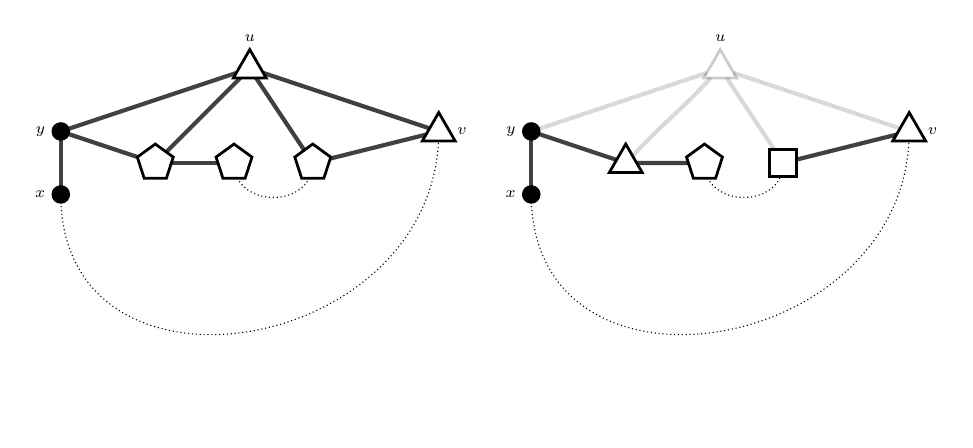
\begin{tikzpicture}
\begin{scope}[scale=0.8, every node/.append style={transform shape}]]
\draw[densely dotted] (3, 1) to [out=270,in=270,looseness=1.5] (-3, 0);
\draw[densely dotted] (-0.25, 0.5) to [out=270,in=270,looseness=1.5] (1.0, 0.5);

\VertexI[label=$x$, position=left, x=-3, y=0]{X}
\VertexI[label=$y$, position=left, x=-3, y=1]{Y}

\VertexIII[label=$u$, position=above, x=0, y=2]{U}
\VertexIII[label=$v$, position=right, x=3, y=1]{V}
\VertexV[x=-1.5, y=0.5]{u1}
\VertexV[x=-0.25, y=0.5]{u2}
\VertexV[x=1.0, y=0.5]{u3}

\Edge(X)(Y)
\Edge(Y)(U)
\Edge(U)(V)
\Edge(Y)(u1)
\Edge(u1)(u2)
\Edge(u3)(V)
\Edge(U)(u1)
\Edge(U)(u3)

\end{scope}

\begin{scope}[xshift=170, scale=0.8, every node/.append style={transform shape}]]
\draw[densely dotted] (3, 1) to [out=270,in=270,looseness=1.5] (-3, 0);
\draw[densely dotted] (-0.25, 0.5) to [out=270,in=270,looseness=1.5] (1.0, 0.5);

\VertexI[label=$x$, position=left, x=-3, y=0]{X}
\VertexI[label=$y$, position=left, x=-3, y=1]{Y}

\Vertex[label=$u$, position=above, x=0, y=2, color=white, style={regular polygon, regular polygon sides=3, opacity=0.2}]{U}
\VertexIII[label=$v$, position=right, x=3, y=1]{V}
\VertexIII[x=-1.5, y=0.5]{u1}
\VertexV[x=-0.25, y=0.5]{u2}
\VertexIV[x=1.0, y=0.5]{u3}

\Edge(X)(Y)
\Edge[opacity=0.2](Y)(U)
\Edge[opacity=0.2](U)(V)
\Edge(Y)(u1)
\Edge(u1)(u2)
\Edge(u3)(V)
\Edge[opacity=0.2](U)(u1)
\Edge[opacity=0.2](U)(u3)

\end{scope}
\end{tikzpicture}
\vspace{-1cm}
\caption{Illustration of Thomassen's reduction. At most $2$ colors are erased from the lists of $u$'s neighbors.}
\end{figure}

\end{proof}

\todo{Criticality definition. Discuss it}

In coloring problems, it is useful to consider when a precoloring of a subgraph
does not \emph{extend} to the entire graph, that is, there is no coloring
of the entire graph under certain constraints which agrees with the coloring 
of the subgraph. 




\begin{definition}[Extending]
	Let $G$ be a graph, $T \subseteq G$ a subgraph, and $L$ a list assignment
	for $G$. For an $L$-coloring $\phi$ of $T$, we say that $\phi$ \emph{extends}
	to an $L$-coloring of $G$ if there exists an $L$-coloring $\psi$ of $G$
s	such that $\phi(v) = \psi(v)$ for all $v \in V(T)$. 
	
\end{definition}

It is also interesting to consider graphs which are critical in this setting. To do so, we use the following definition (from \cite{fivelistcoloring2}):

\begin{definition}[$T$-critical]
	Let $G$, $T$, $L$ be as above. The graph $G$ is \emph{$T$-critical with respect to $L$} if for every proper subgraph $G' \subset G$ such that $T \subseteq G'$, there exists an $L$-coloring of $T$ that extends to an $L$-coloring of $G'$, but does not extend to an $L$-coloring of $G$. If the list assignment $L$ is clear from context, we just say \emph{$T$-critical}.
\end{definition}

\begin{definition}[$\phi$-critical]
	Let, $G$, $T$, $L$ be as above. The graph $G$ is $\phi$-critical for a coloring $\phi$ of $T$ if $\phi$ extends to every proper subgraph of $G$ containing $T$ but not to $G$.
\end{definition}

In a way similar to the general notion of criticality, we have that graphs for which colorings of $T$ do not extend contain a non-trivial $T$-critical subgraph:

\begin{lemma}
Let $G$ be a graph, $T$ a subgraph, and $L$ a list assignment for $G$. If there 
is an $L$-coloring $\phi$ of $T$ that does not extend to $G$, 
then $G$ contains a subgraph $H$ with $T \subsetneq H$ which 
is $\phi$-critical, and hence also $T$-critical with respect 
to $L\restriction_H$. 
\end{lemma}

\begin{proof}
Let $\phi$ be the coloring of $T$ that does not extend and let $H$ be a minimal subgraph 
of $G$ for which $\phi$ does not extend. Now note that $H$ is $\phi$-critical 
by construction.
\end{proof}

\begin{lemma}
\label{minimalsubgraphlemma}
Let $G$ be a graph, $T$ a subgraph, $L$ a list assignment for $G$, and $H \supseteq T$ 
a subgraph of $G$ which is minimal with respect to the following property: 
for every $L$-coloring $\phi$ of $T$ that extends to $H$, $\phi$ also extends to $G$. 
Then $H$ is $T$-critical.
\end{lemma}

\begin{proof}
Suppose not. Then, $H$ contains a proper subgraph $H'$ so that every $L$-coloring $\phi$ that extends to $H'$ also extends to $H$ and hence to $G$. But then $H'$ is a smaller subgraph with that property, contradiction. 
\end{proof}

We also have the following lemma from \cite{fivelistcoloring2}:

\begin{lemma}
\label{pregluinglemma}
Let $T$ be a subgraph of a graph $G$ such that $G$ is $T$-critical with respect to a list assignment $L$. Let $A, B \subseteq G$ be such that $A \cup B = G$ and $T \subseteq A$. Then $G[V(B)]$ is $A[V(A) \cap V(B)]$-critical.
\end{lemma}

\begin{proof} 
Let $G' = G[V(B)]$ and $S = A[V(A) \cap V(B)]$. If $G' = S$ there is nothing to say, suppose otherwise that $G' \neq S$ and note that therefore $G'$ contains an edge not in $S$ (in fact, all isolated vertices of $G'$ must be in $S$). Suppose for a contradiction that $G'$ is not $S$-critical. Then, by taking a maximal proper subgraph that defies the defintion, there exists an edge $e \in E(G') \setminus E(S)$ such that every $L$-coloring of $S$ that extends to $G' \setminus e$ also extends to $G'$. Since $G$ is $T$-critical and $e \not\in E(T)$, there exists a coloring $\phi\restriction_T$ of $T$ that extends to an $L$-coloring $\phi$ of $G \setminus e$, but does not extend to an $L$-coloring of $G$. However, by the choice of $e$, the restriction $\phi\restriction_S$ extends to an $L$-coloring $\phi'$ of $G'$. Let $\phi''$ be such that $\phi''(v) = \phi'(v) \, \forall v \in V(G')$ and $\phi''(v) = \phi(v) \, \forall v \in V(G) \setminus V(G')$. Now, since $A \cup B = G$, $\phi''$ is an $L$-coloring of $G$ extending $\phi\restriction_T$, a contradiction.
\end{proof}

For us, it will be more useful in this form: \todo{check if this is the best phrasing}

\begin{lemma}[Gluing Lemma]
\label{gluinglemma}
Let $T$ be a subgraph of a graph $G$ such that $G$ is $T$-critical with respect to a list assignment $L$. Let $A, B \subseteq G$ be such that $A \cup B = G$. Then $G[V(B)]$ is $(A[V(A) \cap V(B)] \cup T)$-critical.
\end{lemma}

\begin{proof} 
Apply \ref{pregluinglemma} to $A' = A \cup T$ and $B' = B$. 
\end{proof}

\missingfigure{Gluing lemma illustration}

The reason we decided to name it ``Gluing lemma'' in this work is that it is useful to visualize the graph $G$ as made of two separate pieces, $A$ and $B$, which are glued together along $A[V(A) \cap V(B)]$. In our approach we will frequently use the fact that all $T$-critical graphs can be ``decomposed'' in this way. 

\todo{Analogous results for List coloring}




\chapter{Critical Graphs on the Torus}

\todo{Section header}

\section{An Overview of Postle's Approach}

Here we briefly explain Postle's approach in \cite{postlethesis} to obtain the result on the finiteness of 6-list-critical graphs in general surfaces, mentioning specially those intermediate results or definitions we will also use in our approach. The results obtained by Postle are very non-explicit in the sense that the (unspecified) constant in the size bounds for the graphs he obtains is extremely large and hence useless for our purpose of finding an explicit characterization. Nevertheless, given that our approach is primarily guided by this work we consider it of interest to provide a exposition of the main argument.

The results developed in \cite{postlethesis} in 2012 have been published successively in journal articles afterwards, often with improvements in exposition or in the strength of the result. We refer to the corresponding published article in the discussion of each particular result.

\subsection{Notation and Terminology}

Postle works mainly in a setting similar to the hypothesis of Thomassen's stronger theorem: list assignments $L$ which have list sizes of length at least $5$ for interior vertices and at least $3$ for exterior vertices with some exceptions. This setting is encapsulated in the concept of \emph{canvas}.

\begin{definition}[Canvas]
We say that $(G, S, L)$ is a \emph{canvas} if $G$ is a connected plane graph
 with outer walk $C$, $S$ is a subgraph of $C$, and $L$ is a list assignment
  such that $|L(v)| \geq 5 \, \forall v \in V(G) \setminus V(C)$ and
   $|L(v)| \geq 3 \, \forall v \in V(C) \setminus V(S)$. If $S$ is a path,
    we say $(G, S, L)$ is a \emph{path-canvas} or a \emph{wedge}. If $S = C$ and 
    $C$ is a cycle, then $(G, C, L)$ is a \emph{cycle-canvas}.
\end{definition} 



Note: in some places like \cite{fivelistcoloring2}, the term ``canvas'' is used for what Postle calls in \cite{postlethesis} ``cycle-canvas''.

We can restate Thomassen's Stronger Theorem in these terms:

\begin{theorem}
If $(G, P, L)$ is a path-canvas and $|V(P)| \leq 2$, then $G$ is $L$-colorable.
\end{theorem}

\begin{definition}[Critical canvas]
We say that a canvas $(G, S, L)$ is \emph{critical} if it is $S$-critical with respect to $L$.
\end{definition}

It is interesting to study in which circumstances can a critical canvas contain chords or cutvertices.

\todo{determine if I am going to use essential definition}

\begin{definition}

\end{definition}

\begin{lemma}
	If $T = (G, S, L)$ is a critical canvas, then:

	\begin{enumerate}
		\item Every cutvertex of $G$ is essential.
		\item Every chord of the outer walk of $G$ is essential.
	\end{enumerate}
\end{lemma}

\begin{proof}

\end{proof}



\subsection{Variations on Thomassen's Condition}

Much of the technical work on Postle's thesis relies in a careful study of what happens if one varies the condition on \ref{thomassenstrongertheorem}. One of the most elegant (and also useful) results is the following strengthening to Thomassen's Stronger Theorem, originally conjectured by Hutchinson in \cite{hutchinson2012outerplanar}.

\begin{theorem}[Two Lists of Size Two Theorem \cite{fivelistcoloring1}]
\label{twolistsofsizetwo}
If $G$ is a plane graph with outer cycle $C$, $v_1, v_2 \in C$ and $L$ is a list assignment with $|L(v)| \geq 5$ for all $v \in V(G) \setminus V(C)$, $|L(v)| \geq 3$ for all $v \in V(C) \setminus \{v_1, v_2\}$, and $|L(v_1)| = |L(v_2)| = 2$, then $G$ is $L$-colorable. 
\end{theorem}

Or, in the language of canvases:

\begin{theorem}
If $(G, S, L)$ is a canvas with $|V(S)| = 2$ and $L(v) \geq 2$ for $v \in S$, then $G$ is $L$-colorable.
\end{theorem}

This theorem is not true when one of the two vertices has list of size $1$. In fact, Postle characterizes exactly when it fails:

\begin{definition}[Coloring Harmonica]
Let $G$ be a plane graph and $L$ a list assignment for $G$. Given an edge $uv$ and a vertex $w$ both from the outer face of $G$, we say that $(G, L)$ is a \emph{coloring harmonica from $uv$ to $w$} if either:

	\begin{itemize}
		\item $G$ is a triangle with vertex set $\{u, v, w\}$ and $L(u) = L(v) = L(w)$ with $|L(u)| = 2$, or
		\item There exists a vertex $z$ incident with the outer face of $G$ such that $uvz$ is a triangle in $G$, $L(u) = L(v) \subseteq L(z)$, $|L(u)| = |L(v)| = 2$, $|L(z)| = 3$, and the pair $(G', L')$ is a coloring harmonica from $z$ to $w$, where $G'$ is obtained by deleting \textbf{one or both} of the vertices $u$, $v$ and $L'$ is obtained from $L$ by $L'(z) = L(z) \setminus L(u)$ and $L'(x) = L(x)$ for all other vertices $z \neq x \in V(G')$.
	\end{itemize}

	Given two vertices $u, w$ in the outer face of $G$, we say $(G, L)$ is a \emph{coloring harmonica from $u$ to $w$} if there exist vertices $x, y$ incident with the outer face of $G$ such that $uxy$ is a triangle in $G$, $|L(u)| = 1$, $L(x) - L(u) = L(y) - L(u)$, $|L(x)-L(u)|=2$, and $(G', L')$ is a coloring harmonica from $xy$ to $w$, where $G'$ is obtained from $G$ by removing $u$, and $L'$ is obtained from $L$ by seting $L'(x) = L'(y) = L(x)-L(u)$ and $L'(z) = L(z)$ for every $z \in V(G') \setminus \{x, y\}$.


We say that $(G, L)$ is a coloring harmonica if it is a coloring harmonica from $uv$ to $w$ or a coloring harmonica from $u$ to $w$ for some $u, v, w$ as specified earlier.
\end{definition}

\missingfigure{harmonica}

See the example in (reference to figure) (from \cite{fivelistcoloring3}) for some clarity with respect to this mutually recursive definition. Note that the definition makes it clear that graphs which contain a coloring harmonica as a subgraph are not $L$-colorable. 

\begin{theorem}{One List of Size One and One List of Size Two Theorem \cite{fivelistcoloring3}}
Let $G$ be a plane graph with outer cycle $C$, let $p_1, p_2 \in V(C)$, and let
$L$ be a list assignment with $|L(v)| \geq 5$ for all $v \in V(G) \setminus V(C)$, $|L(v)| \geq 3$ for all
$v \in V (C) \setminus \{p_1 , p_2\}$, $|L(p_1)| \geq 1$ and $|L(p_2)| \geq 2$. Then $G$ is $L$-colorable if and only if the pair $(G, L)$ does not contain a coloring harmonica from $p_1$ to $p_2$.
\end{theorem}

Studying conditions of the sizes of the lists in the boundary in which the graph is not $L$-colorable like this one is also useful, because such conditions arise when dealing when reductions and therefore characterizing which are the critical graphs in such settings can give fruitful results.

Thomassen already studied when does the coloring of a path of length $2$ not extend:

\begin{definition}[Bellows]
	We say that a path-canvas $(G, P, L)$ with $P = p_0p_1p_2$ is a \emph{bellows} (terminology from \cite{postlethesis}) or a \emph{generalized wheel} (terminology from \cite{thomassenexponentiallymany5listcolorings}) if either:
	\begin{itemize}
		\item $G$ has no interior vertices and its edge set consists of the edges of the outer cycle plus all edges from $p_1$ to vertices of the outer cycle. In this case, we say that $(G, P, L)$ is a \emph{fan}.
		\item $G$ has one interior vertex $u$ and its edge set consists of the edges of the outer cycle plus all edges from $u$ to vertices of the outer cycle. In this case, we say that $(G, P, L)$ is a \emph{turbofan}.
		\item $G$ can be formed by gluing two smaller bellows from the edges $p_1p_2$ and $p_0p_1$ respectively. 
	\end{itemize}
\end{definition}

\missingfigure{bellows}


\begin{theorem}[\cite{thomassenexponentiallymany5listcolorings}, Theorem 3]
	If $T = (G, P, L)$ is a path-canvas with path length $2$, then $G$ is $L$-colorable unless $T$ has a bellows as a subcanvas.
\end{theorem}

Postle studies when the coloring of two paths of length $1$ does not extend. He finds the following obstruction:

\begin{definition}[Accordion]
	We say that a canvas $T = (G, P_1 \cup P_2, L)$ with $P_1, P_2$ distinct paths of length $1$ is an \emph{accordion} with \emph{ends} $P_1, P_2$ if $T$ is a bellows with $P_1 \cup P_2$ path of length $2$ or $T$ is the gluing of two smaller accordions $T_1 = (G_1, P_1 \cup U, L)$ with ends $P_1, U$ and $T_2 = (G_2, P_2 \cup U, L)$ with ends $U$, $P_2$ along a chord $U = u_1u_2$ where $|L(u_1)|, |L(u_2)| \leq 3$.
\end{definition}

The main result he obtains is that if the two paths are sufficiently far apart, then the graph contains a proportionally large accordion or a coloring harmonica as a subgraph.

\begin{theorem}[Bottleneck Theorem, loosely stated]
\label{bottlenecktheorem}
If $T = (G, P \cup P_0 , L)$ is a canvas with $P, P_0$ distinct edges of $C$ with $d(P, P_0) \geq 14$, then either there exists an $L$-coloring of $G$, or there exists a subcanvas $(G_0 , U_1 \cup U_2 , L)$ of $T$ where $d_{G_0} (U_1, U_2) = \Omega(d_G (P, P_0))$ which is an accordion or a coloring harmonica.
\end{theorem}

This result, along with coloring and structural properties of accordions and harmonicas, is often used as a technical lemma when proving the following results.

\subsection{Linear Bound on Critical Cycle-Canvases}

Postle proves the following result:

\begin{theorem}[\cite{fivelistcoloring2}]
\label{linearboundcycletheorem}
Let $G$ be a plane graph with outer cycle $C$ and $L$ a $5$-lis-assignment for $G$. Let $H$ be a minimal subgraph of $G$ such that every $L$-coloring of $C$ that extends to an $L$-coloring of $H$ also extends to an $L$-coloring of $G$. Then $H$ has at most $19|V(C)|$ vertices.
\end{theorem}

Or, equivalently stated in the language of critical canvases:

\begin{theorem}
If $(G, C, L)$ is a critical cycle-canvas, then $|V(G)| \leq 19 |V(C)|$.
\end{theorem}

The equivalence of the two statements is given by \ref{minimalsubgraphlemma}. This result is interesting in its own right because by \ref{gluinglemma}, all faces of a $T$-critical graph which do not separate vertices from $T$ are in fact critical cycle-canvases, and therefore what the result tells us is that for such graphs there is only finitely many kinds of faces that can appear for each given cycle length. This gives us a lot of information of how critical graphs look like. 

A first observation that can be made is that critical cycle-canvases (in which $C$ is indeed a simple cycle) are $2$-connected, so each face is bounded by a cycle:

\begin{lemma}
If $(G, C, L)$ is a critical cycle-canvas, then it is $2$-connected.
\end{lemma}

\begin{proof}
If $G$ is not $2$-connected, then there exist subgraphs $A, B$ such that $A \cup B = G$ with $|V(A) \cap V(B)| \leq 1$ and $|V(B) \setminus V(A)| \geq 1$. Assume $C \subseteq A$ and apply \ref{gluinglemma} to get that $B$ is $A[V(A) \cap V(B)]$-critical, contradicting \ref{thomassenstrongertheorem}.
\end{proof}

The key result in Postle's proof of the linear bound for cycles is the following theorem about the structure of critical cycle-canvases:

\begin{theorem}[Cycle Chord or Tripod Theorem]
\label{cyclechordtripodtheorem}
If $(G, C, L)$ is a critical cycle-canvas, then either

\begin{enumerate}
\item $C$ has a chord in $G$, or
\item there exists a vertex $v \in V(G) \ V(C)$ with at least three neighbors on $C$ such that at most one of the faces of $G[\{v\} \cup V(C)]$ includes a vertex or edge of $G$. 
\end{enumerate}
\end{theorem}

\todo{think if I should include proof of CCTT}

Using this result, Postle carefully examines what happens near the boundary cycle in order to define some quantities related to sums of lengths of faces and proves that certain inequalities with those quantites are mantained when adding tripods in critical canvases. 



\subsection{The Two Precolored Triangles Theorem}

Next, Postle proves the following theorem:

\begin{theorem}
	There exists $d$ such that the following holds.
	Let $G$ be a planar graph and $T_1, T_2$ triangles in $G$ at distance at least $d$. Let $L$ be a $5$-list-assignment of $G$. Then, every $L$-coloring of $T_1 \cup T_2$ extends to an $L$-coloring of $G$.
\end{theorem}

The value of $d$ that Postle obtains is not explicitly stated, but it is on the order of $100$. However, we conjecture that $4$ or $5$ suffices.

\begin{conjecture}
Let $G$ be a planar graph and $T_1, T_2$ triangles in $G$ at distance at least $5$. Let $L$ be a $5$-list-assignment of $G$. Then, every $L$-coloring of $T_1 \cup T_2$ extends to an $L$-coloring of $G$.
\end{conjecture}

The argument that Postle uses to prove his result is as follows. First, he proves that one can precolor a path between the two triangles in such a way that, when deleting the path and deleting the corresponding colors from the lists of neighboring vertices, all remaining non-precolored vertices have lists of size at least $3$. The proof of this begins with the simple observation that each vertex outside a shortest path has at most $3$ neighbors inside the path. Using planarity properties, a shortest path can be found so that it can be colored in such a way that the vertices with $3$ neighbors inside the path only see two different colors from their lists.

After precoloring and deleting the path between the two triangles, a canvas $(G, P_1 \cup P_2, L)$ is obtained. If there was a precoloring of the triangles that did not extend, then the canvas contains a critical canvas, and by \ref{bottlenecktheorem} it contains a proportionally long accordion or harmonica. Postle proves that this (together with some technical details related to how the path between the triangles was chosen) implies that in the original graph there must be a long chain of separating triangles so that the graph between each separating triangle pertains to one of three very specific types, which he calls tetrahedral, octahedral or hexadecahedral bands. 

\todo{check if I defined separating triangle in introduction}

Finally, he proves that for a sufficiently long chain of this type, any precoloring of the innermost and outermost triangles extends to the whole chain. This proves the theorem, because of the following observation:

\begin{proposition}
	Let $G$ be a plane graph with $L$ a list assignment, $T_1$, $T_2$ 
	two facial triangles with $T_1$ bounding the infinite face of $G$, 
	and $T'_1$, $T'_2$ two triangles such that $T'_1$ is a separating 
	triangle between $T_1$ and $T'_2$ and $T'_2$ is a separating 
	triangle between $T'_1$ and $T_2$. Denote by $G[T'_1, T'_2]$ the 
	subgraph comprised between the two triangles $T'_1, T'_2$.  
	If there exists some $L$-coloring of $T_1 \cup T_2$ that does not 
	extend to $G$, then there exists some $L$-coloring of $T'_1 \cup T'_2$ 
	that does not extend to $G[T'_1, T'_2]$.
\end{proposition}

\begin{proof}
	By \ref{thomassenstrongertheorem}, the coloring on $T_1$ extends to 
	$G[T_1, T'_1]$ and the coloring on $T_2$ extends to $G[T'_2, T_2]$. 
	The coloring of $T'_1 \cup T'_2$ given by this extensions can not 
	extend to $G[T'_1, T'_2]$ by the assumption that the original coloring 
	of $T_1 \cup T_2$ did not extend to $G$.
\end{proof}

\subsection{Hyperbolicity}
\todo{hyperbolicity and cylinder canvases section}

\section{Critical Graphs on the Torus for (usual) Vertex Coloring}

In this section we discuss the result from Thomassen in \cite{thomassentorus} that characterizes the critical graphs for $5$-coloring (not $5$-list-coloring) on the torus.

\subsection{The Critical Graphs}

\begin{theorem}[\cite{thomassentorus}]
	\label{thomassentorustheorem}
	A graph $G$ embeddable on the torus is $5$-colorable if and only if 
	it does not contain the following subgraphs:
	\begin{itemize}
		\item $K_6$.
		\item $C_3 + C_5$.
		\item $K_2 + H_7$, where $H_7$ is the \emph{Moser spindle}, the graph 
		obtained by applying the Hajós construction to a pair of $K_4$. \todo{check if I explained Hajós construction in original}
		\item $T_{11}$, where $T_{11}$ is a triangulation of the torus with $11$ vertices.
	\end{itemize}
	Where $+$ denotes the join of two graphs: their disjoint union with 
	all pairs of vertices from different graphs joined by edges.
\end{theorem} 


\begin{figure}
\centering
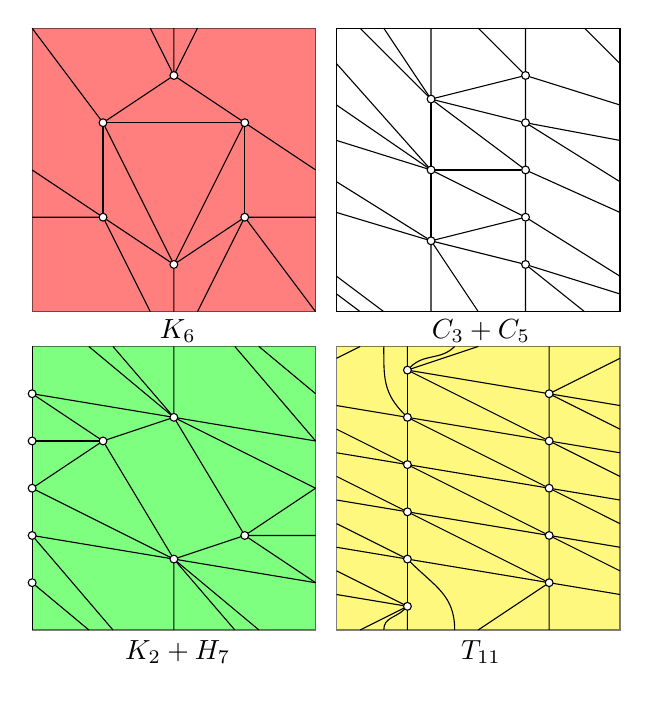
\begin{tikzpicture}[main/.style = {draw, circle, fill=white}]

\begin{scope}[scale=0.3, every node/.append style={transform shape}]]
\draw[draw=black, fill=red, opacity=0.5] (0, 0) rectangle (12, 12);




\node[main] (A1) at (6, 10) {};
\node[main] (A2) at (3, 4) {};
\node[main] (A3) at (9, 4) {};

\node[main] (B1) at (6, 2){};
\node[main] (B2) at (9, 8) {};
\node[main] (B3) at (3, 8) {};


\draw (A1) -- (B2);
\draw (B2) -- (A3);
\draw (A3) -- (B1);
\draw (B1) -- (A2);
\draw (A2) -- (B3);
\draw (B3) -- (A1);

\draw (A1) -- (6, 12);
\draw (6, 0) -- (B1);
%\draw (A2) -- (0, 0);
%\draw (12, 12) -- (B2);
\draw (A3) -- (12, 0);
\draw (0, 12) -- (B3);

\draw (A2) -- (0, 6);
\draw (12, 6) -- (B2);

\draw (B1) -- (B2);
\draw (B2) -- (B3);
\draw (B3) -- (B1);

\draw (A2) -- (0, 4);
\draw (12, 4) -- (A3);
\draw (A2) -- (5, 0);
\draw (5, 12) -- (A1);
\draw (A3) -- (7, 0);
\draw (7, 12) -- (A1);


\end{scope}

\begin{scope}[xshift=110, scale=0.3, every node/.append style={transform shape}]]
\draw[draw=black] (0, 0) rectangle (12, 12);




\node[main] (A1) at (4, 9) {};
\node[main] (A2) at (4, 6) {};
\node[main] (A3) at (4, 3) {};



\node[main] (B1) at (8, 10){};
\node[main] (B2) at (8, 8) {};
\node[main] (B3) at (8, 6) {};
\node[main] (B4) at (8, 4) {};
\node[main] (B5) at (8, 2) {};


\draw (4, 12) -- (A1);
\draw (A1) -- (A2);
\draw (A2) -- (A3);
\draw (A3) -- (4, 0);

\draw (8, 12) -- (B1);
\draw (B1) -- (B2);
\draw (B2) -- (B3);
\draw (B3) -- (B4);
\draw (B4) -- (B5);
\draw (B5) -- (8, 0);

\draw (A1) -- (B1);
\draw (A1) -- (B2);
\draw (A1) -- (B3);
\draw (A1) -- (2, 12);
\draw (2, 0) -- (0, 1.5);
\draw (12, 1.5) -- (B4);
\draw (A1) -- (1, 12);
\draw (1, 0) -- (0, 0.75);
\draw (12, 0.75) -- (B5);

\draw (A2) -- (B3);
\draw (A2) -- (B4);
\draw (A2) -- (0, 10.5);
\draw (12, 10.5) -- (10.5, 12);
\draw (10.5, 0) -- (B5);
\draw (A2) -- (0, 8.75);
\draw (12, 8.75) -- (B1);
\draw (A2) -- (0, 7.25);
\draw (12, 7.25) -- (B2);


\draw (A3) -- (B4);
\draw (A3) -- (B5);
\draw (A3) -- (6, 0);
\draw (6, 12) -- (B1);
\draw (A3) -- (0, 5.5);
\draw (12, 5.5) -- (B2);
\draw (A3) -- (0, 4.2);
\draw (12, 4.2) -- (B3);

\end{scope}


\begin{scope}[yshift=-115, scale=0.3, every node/.append style={transform shape}]]
\draw[draw=black, fill=green, opacity=0.5] (0, 0) rectangle (12, 12);




\node[main] (A1) at (0, 8) {};
\node[main] (A2) at (0, 10) {};
\node[main] (A3) at (0, 2) {};
\node[main] (A4) at (0, 4) {};
\node[main] (A5) at (0, 6) {};

\coordinate[] (A1c) at (12, 8) {};
\coordinate[] (A2c) at (12, 10) {};
\coordinate[] (A3c) at (12, 2) {};
\coordinate[] (A4c) at (12, 4) {};
\coordinate[] (A5c) at (12, 6) {};

\node[main] (H1) at (3, 8) {};
\node[main] (H2) at (9, 4) {};

\node[main] (K1) at (6, 9) {};
\node[main] (K2) at (6, 3) {};




\draw (A1) -- (A2);
\draw (A2) -- (0, 12);
\draw (0, 0) -- (A3);
\draw (A3) -- (A4);
\draw (A4) -- (A5);
\draw (A5) -- (A1);

\draw (H1) -- (A1);
\draw (H1) -- (A2);
\draw (H1) -- (A5);

\draw (H2) -- (A3c);
\draw (H2) -- (A4c);
\draw (H2) -- (A5c);

\draw (K1) -- (A2);
\draw (K1) -- (A1c);
\draw (K1) -- (A5c);
\draw (K1) -- (H1);
\draw (K1) -- (H2);
\draw (K1) -- (3.42, 12);
\draw (3.42, 0) -- (A4);
\draw (K1) -- (2.4, 12);
\draw (2.4, 0) -- (A3);

\draw (K2) -- (A5);
\draw (K2) -- (A4);
\draw (K2) -- (A3c);
\draw (K2) -- (H1);
\draw (K2) -- (H2);
\draw (K2) -- (12-3.42, 0);
\draw (12-3.42, 12) -- (A1c);
\draw (K2) -- (12-2.4, 0);
\draw (12-2.4, 12) -- (A2c);


\draw (K1) -- (6, 12);
\draw (6, 0) -- (K2);
\end{scope}

\begin{scope}[xshift=110, yshift=-115, scale=0.3, every node/.append style={transform shape}]]
\draw[draw=black, fill=yellow, opacity=0.5] (0, 0) rectangle (12, 12);




\node[main] (A0) at (3, 11) {};
\node[main] (A1) at (3, 9) {};
\node[main] (A2) at (3, 7) {};
\node[main] (A3) at (3, 5) {};
\node[main] (A4) at (3, 3) {};
\node[main] (A5) at (3, 1) {};

\node[main] (B0) at (9, 10) {};
\node[main] (B1) at (9, 8) {};
\node[main] (B2) at (9, 6) {};
\node[main] (B3) at (9, 4) {};
\node[main] (B4) at (9, 2) {};

\draw (A0) -- (A1);
\draw (A1) -- (A2);
\draw (A2) -- (A3);
\draw (A3) -- (A4);
\draw (A4) -- (A5);

\draw (B0) -- (B1);
\draw (B1) -- (B2);
\draw (B2) -- (B3);
\draw (B3) -- (B4);

\draw (A0) -- (B0);
\draw (A0) -- (B1);
\draw (A1) -- (B1);
\draw (A1) -- (B2);
\draw (A2) -- (B2);
\draw (A2) -- (B3);
\draw (A3) -- (B3);
\draw (A3) -- (B4);
\draw (A4) -- (B4);

\draw (B0) -- (12, 9.5);
\draw (0, 9.5) -- (A1);
\draw (B0) -- (12, 8.5);
\draw (0, 8.5) -- (A2);
\draw (B1) -- (12, 7.5);
\draw (0, 7.5) -- (A2);
\draw (B1) -- (12, 6.5);
\draw (0, 6.5) -- (A3);
\draw (B2) -- (12, 5.5);
\draw (0, 5.5) -- (A3);
\draw (B2) -- (12, 4.5);
\draw (0, 4.5) -- (A4);
\draw (B3) -- (12, 3.5);
\draw (0, 3.5) -- (A4);
\draw (B3) -- (12, 2.5);
\draw (0, 2.5) -- (A5);
\draw (B4) -- (12, 1.5);
\draw (0, 1.5) -- (A5);

\draw (A4) to [out=-45, in=90, looseness=1.1] (5, 0);

\draw (5, 12) to [out = -135, in = 45, looseness=1.05] (A0);

\draw (B4) -- (6, 0);
\draw (6, 12) -- (A0);
\draw (B4) -- (9, 0);
\draw (9, 12) -- (B0);

\draw (A5) -- (3, 0);
\draw (3, 12) -- (A0);
\draw (A5) to [out=-135, in = 90, looseness=1.1] (2, 0);
\draw (2, 12) to [out=-90, in =135, looseness=1.1] (A1);
\draw (A5) -- (1, 0);
\draw (1, 12) -- (0, 11.5);
\draw (12, 11.5) -- (B0);

\end{scope}

\node[] at (1.85, -0.25) {$K_6$};
\node[] at (5.70, -0.25) {$C_3+C_5$};
\node[] at (1.85, -4.32) {$K_2+H_7$};
\node[] at (5.70, -4.32) {$T_{11}$};
\end{tikzpicture}
\caption{$6$-critical graphs embedded on the torus.}
\end{figure}

If a graph is not $5$-colorable, it is not $5$-list-colorable, so all graphs 
that contain any of the above subgraphs are not $5$-list-colorable. 
We conjecture that this characterizes the $5$-list-colorable graphs on the torus too:

\begin{conjecture}
\label{torusconjecture}
A graph $G$ embeddable on the torus is $5$-list-colorable if and only if 
it does not contain the following subgraphs: $K_6$, $C_3 + C_5$, $K_2 + H_7$, $T_{11}$.
\end{conjecture}

This means that those are the minimal $6$-list-critical graphs on the torus. Note 
that there may be additional $6$-list-critical graphs embeddable on the torus, but what we are conjecturing is that they all 
contain those subgraphs. For example:

\begin{observation}
$K_7$ is $6$-list-critical.
\end{observation}

\begin{proof}
Consider the following $5$-list-assignment for $K_7$: $L(v_1) = L(v_2) = L(v_3) = L(v_4) = L(v_5) = \{1, 2, 3, 4, 5\}$, 
$L(v_6) = L(v_7) = \{1, 2, 3, 4, 6\}$. $K_7$ is not $L$-colorable, since there are only $6$ available colors. 
But any subgraph is $L$-colorable. Let's give a coloring $\phi$ for $K_7 \setminus v_iv_j$. If $i, j \leq 5$, 
then setting $\phi(v_i) = \phi(v_j) = 5$ and $\phi(v_7) = 6$ leaves $4$ vertices to be colored with $4$ colors. 
If $i \leq 5$ and $j \geq 6$, then setting $\phi(v_i) = \phi(v_j) = 1$, $\phi(v_{13-j}) = 6$ leaves $4$ vertices 
to be colored with $4$ colors. If $\{i, j\} = \{6, 7\}$, then $\phi(v_i) = \phi(v_j) = 6$ leaves $5$ vertices 
to be colored with $5$ colors.

Hence, $K_7$ is $L$-critical for a $5$-list-assignment $L$, and is therefore $6$-list-critical.
\end{proof}

\subsection{An Overview of Thomassen's Approach}

Thomassen's article where he characterizes the graphs on the torus (\cite{thomassentorus}) predates 
his result on finitely many $6$-critical graphs for all surfaces (\cite{thomassenfixedsurface}). 
For the characterization of $6$-critical graphs on the torus, he only uses elementary, relatively 
straighforward arguments that work on specifically in the torus. We briefly summarize his 
approach here in order to discuss which arguments can be reused for the list-coloring case. 

First, Thomassen considers the case when the minimum degree is at least $6$. 
He obtains this result:

\begin{theorem}
Let $G$ be a graph embedded on the torus with $\delta(G) \geq 6$. Then $G$ is $5$-colorable 
unless $G = K_7$ or $G = T_{11}$.
\end{theorem}

We will discuss later how to arrive at this result, because this is the part of the proof that 
can be adapted for list-coloring. But let us first describe Thomassen's argument for 
general graphs.

He assumes a minimum counterexample $G_0$ to \ref{thomassentorustheorem} (the counterexample has
minimum number of vertices, maximum number of edges restricted to that, and some other assumptions 
about details we will not discuss here). By the previous result, 
there must be a vertex $v_0 \in V(G_0)$ with degree $\leq 5$, and the degree of $v_0$ is in 
fact equal to $5$ by minimality of the counterexample. 

Consider two vertices $x, y \in N(v_0)$ which are not adjacent (if all the vertices of 
$N(v_0)$ were adjacent, then $G_0$ would contain $K_6$, a contradiction). Let $G_{xy}$ be 
the graph obtained from $G_0 \setminus v_0$ by identifying the vertices $x$ and $y$. 
$G_{xy}$ can be embedded in the torus by modifying the embedding of $G_0$. If $G_{xy}$ 
were $5$-colorable, then we would have a $5$-coloring of $G_0$ by assigning the same color 
to $x$ and $y$ and coloring $v_0$ with a color not appearing in its $5$ neighbors. 
Hence, $G_{xy}$ is not $5$-colorable and by minimality of our counterexample it 
contains $K_6$, $C_3 + C_5$, $K_2 + H_7$ or $T_{11}$.

The above argument works for all pairs $x, y$ of non-adjacent vertices in $N(v_0)$, so potentially 
we can have many different obstructions for each of the corresponding $G_{xy}$ subgraphs. 
But we can prove that, by minimality, there can not be much else in $G_0$ apart from these
obstructions arising from all the $G_{xy}$ subgraphs. More precisely:  

\begin{proposition}
	\label{g0proposition}
	For any non-adjacent $x, y \in N(v_0)$, let $G'_{xy}$ a copy of 
	$K_6$, $C_3 + C_5$, $K_2 + H_7$ or $T_{11}$ in $G_{xy}$, and let $G''_{xy}$ be the induced
	subgraph of $G_{xy}$ by the vertex set of $G'_{xy}$. Then $G_0$ consists of $v_0$, $N(v_0)$, 
	the edges between vertices of $\{v_0\} \cup N(v_0)$, and the union over all non-adjacent 
	$x, y \in N(v_0)$ of the graph obtained from $G''_{xy}$ by splitting the contracted vertex
	into $x$ and $y$.  
\end{proposition}

\begin{proof}
We will prove that the graph described above, which is a subgraph of $G_0$, is not $5$-colorable. 
This means, by the assumptions of minimality of vertices and maximality of edges, that $G_0$ is
in fact equal to that subgraph. 

If the subgraph had a $5$-coloring, then two non-adjacent vertices $x, y$ of $N(v_0)$ would 
have the same color. But by then identifying the two vertices we can get a $5$-coloring 
of $G''_{xy}$, which contains the non-$5$-colorable subgraph $G'_{xy}$, contradiction.

\end{proof}

Note that, since the maximum number of vertices in a critical graph is $11$, this means that
$G_0$ has at most $(11 - 1) \cdot \binom{5}{2} + 6 = 106$ vertices, and hence what remains
is a finite problem.

Thomassen uses some more arguments to narrow down the remaining possibilities for $G_0$, but
we can already see an important point of failure of this argument for list-coloring: in the 
proof of \ref{g0proposition}, it is used that a necessary and sufficient condition for a coloring
of $G_0 \setminus v_0$ to extend to $v_0$ is that two neighbors of $v_0$ have the same color.
In list coloring, this condition is not necessary. So we cannot conclude that the minimum 
counterexample is the union of the graphs induced by the obstructions in $G_{xy}$ and the 
argument breaks down here. 



\subsection{$6$-Regular $6$-Critical Graphs}

As we said before, Thomassen's argument for graphs with minimum degree $6$ can be reused for list-coloring. This is because these graphs are very restricted, and therefore their structure can be completely characterized and a $5$-(list)-coloring can be explicitly exhibited for the ones that are colorable. The basic result is this.

\begin{proposition}
If a graph $G$ embedded on the torus has $\delta(G) \geq 6$, then:

\begin{enumerate}
	\item $G$ is $6$-regular.
	\item $G$ is a triangulation of the torus.
\end{enumerate}
\end{proposition}

\begin{proof}
We apply Euler's formula: let $V, E, F$ be the number of vertices, edges and faces in the embedding, respectively. 
We have that $\delta(G) \geq 6 \implies V \leq \frac{1}{3} E$ with equality iff $G$ is $6$-regular, and $F \leq \frac{2}{3}E$ 
with equality iff $G$ is a triangulation. Then $0 = V - E + F \leq \frac{1}{3}E - E + \frac{2}{3}E = 0$, so we have equality on both inequalities.
\end{proof}

Using the proposition above, Thomassen then proves the following:

\begin{proposition}[3.2 in \cite{thomassentorus}]
Let $G$ be a $6$-regular graph on the torus. If $G$ contains a vertex $v$, such that $\{v\} \cup N(v)$ induces a nonplanar graph, then $G = K_7$ or $G$ is obtained from $K_8$ or $K_9$ by deleting the edges of a $1$-regular or $2$-regular subgraph.
\end{proposition}

The study of $6$-regular graphs on the torus without vertices whose neighborhood induces a nonplanar graph was already done by Thomassen in his previous paper \cite{thomassentilings}, in the context of finding all tilings of the torus in order to prove a conjecture by Babai about vertex-transitive graphs. 


\todo{finish 6-regular graphs section}
 see if it is worth it to include, maybe it is nontrivial to actually prove 5-list-colorability




\section{Our Approach}


\section{Generation of Critical Graphs}

In this section we describe algorithms for processing and generating critical canvases via computer search.

\subsection{Representation of Canvases}

The first step is deciding how to represent canvases in our algorithms. Recall that a canvas $T$ is a tuple 
$(G, S, L)$ where $G$ is a plane graph, $S$ is a subgraph of the outer face and $L$ is a list assignment for 
$G$ satisfying some conditions. Here, in each algorithm we will usually be working with one particular family of 
canvases at a time, for example cycle-canvases or path-canvases with a fixed size of cycle or path, so the 
information about the subgraph $S$ can be ``implicit'' in each different representation for each different algorithm
instead of working with a general representation that allows all canvases. Also, in some scenarios we will be 
working with conditions on the list assignment $L$ which are different from the ones in the definition of canvas.
In this section we intend to just expose some general ideas about how the representation of graphs in this context
can be done, which will be afterwards applied in different scenarios.

The most important thing to state is that we will not be interested in storing the list assignment $L$ at all. 
This is because there is a significant combinatorial explosion in the number of list assignments to be considered and
we are interested in the graphs themselves, not the list assignments. Also, most of the results
we will be using such as \ref{gluinglemma} or \ref{cyclechordtripodtheorem} are directly related to subgraphs
and not list assignments, and while they are in theory stated with respect to a fixed list assignment, it is more
useful in practice to not consider the list assignment at all. 

Thus, when we generate all critical canvases $(G, S, L)$, what we will actually be doing is generate all pairs $(G, S)$ 
such that there exists some list assignment $L$  so that $(G, S, L)$ is a critical canvas. In some scenarios, we will also
be interested in storing the prescribed size of the list assignment for each vertex: that is, we will be storing a tuple $(G, S, f)$
with $f : V(G) \rightarrow \mathbb{N}$ so that we will only be considering list assignments $L$ with $|L(v)| = f(v)$, but other
than that we will not store information about the actual list assignment. 

We store the information of the graph $G$ with an adjacency list. We will also be interested in storing the planar embedding of the graph:
to do so, we order the edges in the adjacency list of each vertex according to their clockwise order in the embedding (as in a
\emph{rotation system}). This information, together with the information of which vertices are in the outer face, is enough to reconstruct
the embedding. 

We will want to test when two canvases are isomorphic. More generally, we will want to have a canonical form for each canvas, so that
given a set of canvases $\mathcal{S}$ and a new canvas $T$, we can check whether there is a canvas isomorphic to $T$ in $\mathcal{S}$ by checking the 
presence of the corresponding canonical form of $T$ in an associative array with the canonical forms of the canvases in $\mathcal{S}$.


...

\subsection{Generation of Critical Cycle-Canvases}

Our algorithm for the generation of critical cycle-canvases is based on \ref{cyclechordtripodtheorem}. 
This theorem says that every critical cycle-canvas can either be decomposed into two smaller critical 
cycle-canvases through a chord in the outer face, it can be decomposed into a ``tripod'', a vertex $v$ 
with at least $3$ neighbors in $C$, and a smaller critical cycle-canvas contained in the only nonempty 
face incident with $v$. In these decompositions, it is possible that instead of a smaller critical canvas 
we get an empty canvas, which is technically not critical. \todo{check that all definitions of critical 
canvases are consistent with this}

This implies that we can generate all critical cycle-canvases from smaller cycle-canvases by gluing
cycle-canvases through outer face edges to get a canvas with a chord, or by adding a tripod to the
outside of a cycle-canvas. We then have to check whether the resulting canvas is indeed critical,
since the decomposition into two smaller critical cycle-canvases is a necessary but not sufficient condition
for criticality. We will see how to do this in Section 4. \todo{references for sections}.

\missingfigure{The three cases for generation of critical cycle-canvases}

\todo{figure for generation of critical cycle-canvases and references to figure}

If we are generating cycle-canvases with cycle length $\ell$, then a chord partitions
the cycle-canvas into two cycle-canvases of length $a$, $b$ with $a, b \geq 3$ and $a + b = \ell + 2$ (see figure (a)), so 
$a, b \leq \ell-1$ and therefore if we have generated all cycle-canvases with cycle length $< \ell$ we can generate
all cycle-canvases with cycle length $\ell$ with a chord. In the case of adding a tripod, though, if the vertex $v$ of
the tripod is adjacent to only three adjacent vertices in the outer face, then the smaller cycle-canvas has the same
cycle length as the larger cycle-canvas (see figure (c)).

In order to resolve this, what we do is first generate all the cycle-canvases obtained from cycle-canvases with smaller cycle size 
(as in figure (a) and (b)), enqueue the resulting critical canvases, and then process the canvases from the queue and add tripods 
to three consecutive vertices in all possible ways, enqueueing the new critical cycle-canvases that are found. Here is the description 
of the algorithm:

\begin{algorithm}[H]
\caption{Generation of Critical Cycle-Canvases.}
\SetAlgoLined
\SetKwComment{Comment}{/* }{ */}
\SetKwProg{Fn}{function}{}{end}
\Comment*[h]{Generate critical canvases of cycle size $\ell$, including empty one}

\Fn{generateCriticalCycleCanvases($\ell$)}{ 
	
	\For{$i = 3, \ldots, \ell-1$} {
		$S_i \gets \text{generateCriticalCycleCanvases}(i)$\;
	}
	$S \gets \{ \text{emptyCycle}(\ell) \}$\;
	
	\For{$a = 3, \ldots, \ell-1$} {
		$b \gets \ell-a+2$\;
		\For{$G_1 \in S_a$} {
			\For{$G_2 \in S_b$} {
				$T \gets \text{fuseChordSet}(G_1, G_2)$\; 
				\Comment*[r]{Set of cycle-canvases obtained by fusing $G_1$ and $G_2$ along outer cycle edges in all possible ways}
				\For{$G \in T$} {
					\If{$G \not\in S$ AND $\text{isCritical}(G)$} {	
						$S \gets S \cup \{G\}$\;
					}
				} 
			}
		}
	}
	\For{$k = 3, \ldots, \ell-1$} {
		\For{$G_1 \in S_k$} {
			$T \gets \text{addTripodSet}(G_1, \ell-k+3, 3)$\;
			\Comment*[r]{Set of cycle-canvases obtained by adding a tripod with $3$ neighbors in the outer face to get a cycle-canvas of length $\ell$ in all possible ways}
			\For{$G \in T$} {
				\If{$G \not\in S$ AND $\text{isCritical}(G)$} {	
					$S \gets S \cup \{G\}$\;
				}
			} 
		}
	}	
	$Q \gets \text{Queue}(S)$\; 
	\While{$Q \text{ is not empty}$} {
		$G_1 \gets \text{first}(Q)$\;
		$\text{dequeue}(Q)$\;
		$T \gets \text{addTripodSet}(G_1, 3, 3)$\;
		\For{$G \in T$} {
			\If{$G \not\in S$ AND $\text{isCritical}(G)$} {	
				$S \gets S \cup \{G\}$\;
				$\text{enqueue}(Q, G)$\;
			}
		} 
	}
	return $S$\;
}


\end{algorithm}

\todo{fix algorithm size}


Note that we only need to add tripods with $3$ adjacent neighbors since vertices with a larger number of neighbors in the
outer face can be obtained by first adding chords and then adding finally adding a tripod with $3$ neighbors. However, 
often we are interested in just generating chordless critical canvases. In that case, we do need to add tripods of all sizes.
The modified algorithm for chordless critical cycle-canvases is the following:

\begin{algorithm}[H]
\caption{Generation of Chordless Critical Cycle-Canvases.}
\SetAlgoLined
\SetKwComment{Comment}{/* }{ */}
\SetKwProg{Fn}{function}{}{end}
\Comment*[h]{Generate critical canvases of cycle size $\ell$, including empty one}

\Fn{generateCriticalCycleCanvases($\ell$)}{ 
	
	\For{$i = 3, \ldots, \ell-1$} {
		$S_i \gets \text{generateCriticalCycleCanvases}(i)$\;
	}
	$S \gets \{ \text{emptyCycle}(\ell) \}$\;
	\For{$k = 3, \ldots, \ell-1$} {
		\For{$j = 3, \ldots, \ell-k+3$} {
			\For{$G_1 \in S_k$} {
				$T \gets \text{addTripodSet}(G_1, \ell-k+3, j)$\;
				\For{$G \in T$} {
					\If{$G \not\in S$ AND $\text{isCritical}(G)$} {	
						$S \gets S \cup \{G\}$\;
					}
				} 
			}
		}
	}	
	$Q \gets \text{Queue}(S)$\; 
	\While{$Q \text{ is not empty}$} {
		$G_1 \gets \text{first}(Q)$\;
		$\text{dequeue}(Q)$\;
		$T \gets \text{addTripodSet}(G_1, 3, 3)$\;
		\For{$G \in T$} {
			\If{$G \not\in S$ AND $\text{isCritical}(G)$} {	
				$S \gets S \cup \{G\}$\;
				$\text{enqueue}(Q, G)$\;
			}
		} 
	}
	return $S$\;
}


\end{algorithm}


\subsection{Generation of Critical Wedges}

\todo{Generation of critical wedges: chord or tripod theorem, etc}



\section{Criticality Testing}

In this section we describe algorithms used to determine list-criticality of graphs. Recall that we are not storing the explicit list assignment $L$ for our graphs, so what we want to check is whether there exists a $L$ so that the graph is critical with respect to that $L$. However, even if $L$ was fixed, it would still be a computationally hard problem to determine criticality. What we will do instead is check for weaker properties, and therefore admit some false positives, that is, some graphs we identify as list-critical for which actually no suitable $L$ exist. Our hope is that the tests will be exhaustive enough so that finiteness results such as \ref{linearboundcycletheorem} still hold for the weaker properties we are testing, and our algorithms terminate. We will see that indeed, the algorithms described here work very well in practice at discarding non-critical graphs. 

\todo{explain that we work with graphs with prescribed list sizes}

\subsection{Degree properties}

We can start with an easy observation:

\begin{Observation}
In a $L$-critical graph, $d(v) \geq |L(v)|$ for all vertices $v$.
\end{Observation}

So if we find a vertex with degree less than the prescribed list size, we can conclude that the graph is not list-critical. 
However, this is a very weak test. We can incorporate another test concerning the vertices with $d(v) = |L(v)|$: there is
the following result by Gallai showing that the subgraph induced by those vertices must have a certain structure, generalizing 
the classical Brooks theorem for vertex coloring:

\begin{theorem}[Gallai \cite{gallaikritische}]
Let $G$ be a $L$-critical graph and let $H$ be the subgraph
of $H$ induced by the vertices with $d(v) = |L(v)|$. 
Then each $2$-connected component of $H$ is a complete graph or an odd cycle.
\end{theorem}

\subsection{Reducible Configurations}

\begin{figure}
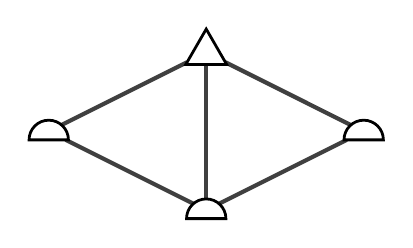
\begin{tikzpicture}
	\VertexIII[y=1]{A}
	\VertexII[x=-2]{B}
	\VertexII[y=-1]{C}
	\VertexII[x=2]{D}
	
	\Edge(A)(B)
	\Edge(A)(C)
	\Edge(A)(D)
	\Edge(B)(C)
	\Edge(C)(D)
\end{tikzpicture}
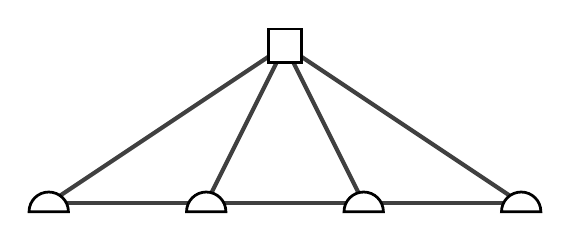
\begin{tikzpicture}
	\VertexIV[y=1]{X}
	\VertexII[x=-3, y=-1]{A}
	\VertexII[x=-1, y=-1]{B}
	\VertexII[x=1, y=-1]{C}
	\VertexII[x=3, y=-1]{D}
	
	\Edge(X)(A)
	\Edge(X)(B)
	\Edge(X)(C)
	\Edge(X)(D)
	\Edge(A)(B)
	\Edge(B)(C)
	\Edge(C)(D)
\end{tikzpicture}
\end{figure}

\subsection{The Alon-Tarsi Method}
\subsection{Recursive Colorability Testing}

\begin{algorithm}[H]
\caption{Recursive Colorability Testing.}
\SetAlgoLined
\SetKwProg{Fn}{function}{}{end}
\Fn{containsColorableSubgraph(G)}{
\If{$G$ is empty} {
	return false\;
}
\If{alonTarsi($G$)} {
	return true\;
}
$H \gets \text{minimalNonColorable}(G)$\;
return containsColorableSubgraph($G \setminus H$)\;
}
\Fn{minimalNonColorable(G)}{
	\For{$v \in V(G)$} {
		\If{not alonTarsi(removeVertex($G$,$v$))} {
			return minimalNonColorable(removeVertex($G$,$v$))\;
		}
	}
	return $G$\;
}


\end{algorithm}
\subsection{Criticality Verification}


\section{Approaches to the Two Precolored Triangles Theorem}

\subsection{Canvas Strangulation}

\subsection{The Forbidden 3-3 Reduction}

\subsection{Criticality Strength}


\section{Conclusions and Further Study}

\newpage

\todo{fix bibliography (not arxiv version, extraneous urls, etc}

\printbibliography
\end{document}


